\documentclass[../../diss.tex]{subfiles}
\begin{document}

\section{Valence games}%
\label{Section:ValenceGames}%

The goal of this chapter is to classify the decidability of several types of games on the configuration graphs of valence systems over graph monoids based on the underlying graph structure.
We will tackle this challenge in this section.
We consider games with reachability and coverability as the winning conditions.
In both cases, we show that the only decidable cases are the context-free games that we have studied extensively in \cref{Chapter:ContextFreeGames} and closely related games that can be reduced to context-free ones.

\paragraph{Reachability games on valence systems}

We start by giving a formal definition of valence games.
Consider a valence system in which the set of control states $Q = Q_\allplayer \dotcup Q_\explayer$ is partitioned into the set $Q_\allplayer$ of states owned by the universal player and the set $Q_\explayer$ of states owned by the existential player.
We usually write such a system as \( (\graphmonoid, Q_\allplayer \dotcup Q_\explayer, \delta, \qinit, \qfinal) \) and call it a \emph{game valence system} (over the graph monoid of $G$).
From this definition, we obtain a game arena on the induced transition system as described in \cref{Chapter:Games}.
The configurations owned by the existential player are all configurations $(q,m)$ where the control stated is owned by the existential player, $q \in Q_\explayer$, independent of the storage value, similar for the universal player.
Moves in the game are defined as before: $(q,m) \to (q',m'')$ if there is a transition $q \tow{m'} q'$ in $\delta$ so that $m'' = m \cdot m'$ and $m''$ is right invertible.

A game valence system fixes a game arena.
To obtain a game, it remains to equip this game arena with a winning condition.
For now, we focus on \emph{valence reachability games} in which, starting from $(q_\init,\eps)$, the goal of the existential player is to reach $(\qfinal,\eps)$.
Here, $\eps$ denotes its equivalence class, the neutral element of the monoid.
This means we start in the initial configuration consisting of the initial control state with empty storage and we want to reach the final state with empty storage.
Note that reachability here should be understood as \emph{configuration reachability}, \ie we fix both the target control state and the target storage value, in contrast to control-state reachability games which we will consider later.

All reachability games are known to be positionally determined by the Borel determinacy theorem~\cite{Martin75}.
Hence, we know that for our fixed initial position, exactly one of the players has a winning strategy.
The key problem is computing this winner.
As with context-free games and higher-order games, we are dealing with a situation in which we have to compute information about a game on a potentially infinite game arena based on the finite syntax generating it.

Formally, the problem of solving valence reachability games is defined as follows.

\begin{problem}
    \problemtitle{Solving valence reachability games}
    \probleminput{Game valence system $(\graphmonoid,Q_\allplayer \dotcup Q_\explayer, \delta, \qinit, \qfinal)$.}
    \problemquestion{Can the existential player enforce visiting $(q_\final,\eps)$ from $(q_\init,\eps)$?}
\end{problem}

\begin{remark*}
    When defining the semantics of valence systems, we have introduced the right-invertibility restriction: We can only apply a transition $q \tow{m'} q'$ in configuration $(q,m)$ if $m \cdot m'$ is right invertible.
    The justification for this restriction was the fact that if $m \cdot m'$ is not right invertible, then it will be impossible to reach $(q_\final,\eps)$ from $(q',m \cdot m')$.
    However, for the answer to the reachability problem, it is irrelevant whether we allow transitions to non-right-invertible storage values.
    We are only considering existential nondeterminism in this case, so the existence of additional transitions that are not helpful does not matter.
    This is different in the case of valence games.
    If the universal player would be allowed to take a transition leading to a non-right-invertible storage value, the result is a configuration from which the existential player cannot win.
    Transitions to non-right-invertible values typically correspond to illegal operations on the storage, \eg a pop-operation that pops a symbol that is not the current top-of-stack.
    Hence, it is important to forbid these transitions to obtain the desired semantics for valence reachability games.
\end{remark*}

Valence reachability games can be seen as an extension of the reachability problem for valence systems; the latter corresponds to games in which all control-states are owned by the existential player.
If the graph $G$ contains $C_4$ from \cref{Figure:ValenceSystemExamplesC4} or $P_4$ from \cref{Figure:ValenceSystemExamplesP4} as an induced subgraph, then reachability in a non-game setting is undecidable~\cite{Zetzsche21}.
Since reachability games are a generalization of the reachability problem for valence systems, we immediately obtain that valence reachability games are undecidable in this case.
Hence, there is no hope for valence reachability games being solvable in general.
As typical for valence systems, we study instead for which graphs $G$ valence reachability games over that graph are decidable.
We formalize this in the form of the following version of the decidability problem in which the underlying graph is fixed.

\begin{problem}
    \problemtitle{Solving valence reachability games over graph $G$}
    \probleminput{Game valence system $(\graphmonoid,Q_\allplayer \dotcup Q_\explayer, \delta, \qinit, \qfinal)$ where $\graphmonoid$ is induced by $G$.}
    \problemquestion{Can the existential player enforce visiting $(q_\final,\eps)$ from $(q_\init,\eps)$?}
\end{problem}

We already know some graphs $G$ for which valence reachability games will be decidable.
We have argued before that graphs that do not contain any edge correspond to pushdown systems, where the number of nodes in the graph corresponds to the number of stack symbols.
The graph from \cref{Figure:ValenceSystemExamplesPDS} is one such example.
Valence reachability games for such graphs are essentially pushdown games, a type of context-free games.
We have extensively discussed the decidability of such games \cref{Chapter:ContextFreeGames}, see in particular \cref{Section:CFGamesRelWork} for algorithms that can directly deal with pushdown games.

Our main result in this part of the section is that this is essentially the only case in which valence reachability games are decidable.
To make this precise, we introduce some notation.
We will see later that the existence of self-loops does not influence the decidability of reachability games.
We denote by $\irreflexive{G}$ the \emph{irreflexive version of $G$}, $G$ with all self-loops removed.
Formally, if $G = (V,I)$, then $\irreflexive{G} = (V, I \setminus \Set{ (o,o)}{o \in V})$.
Our classification will characterize decidability depending on~$\irreflexive{G}$ rather than on $G$ itself.

We call a graph a \emph{pushdown graph} if it contains no edges among distinct nodes.
Graph $G$ is a pushdown graph iff $\irreflexive{G}$ contains no edge at all.
Our main result states that pushdown graphs are exactly the graphs for which valence reachability games are decidable.

\begin{theorem}%
\label{Theorem:ValenceReachabilityGamesClassification}%
    Valence reachability games over graph $G$ are decidable if and only if $G$ is a pushdown graph.
\end{theorem}

The proof of the result is split into two parts.
We first use the decidability of context-free games to show that valence reachability games over pushdown graphs are decidable.
For the other direction, we show that if $\irreflexive{G}$ contains an edge, then the class of valence reachability games over $G$ are not decidable.

\paragraph{Valence reachability games -- The decidable case}

Let us treat the decidable case first.
We start with considering a simple case.
If $G$ contains no edge at all, in particular if it contains no self-loops, then we have $G = \irreflexive{G}$.
It is straightforward to see a valence reachability game over $G$ as a context-free game defined by a pushdown automaton.
We see transitions labeled by $\inc{a}$ as transitions labeled by $\pushop a$, similar for $\dec{a}$ and $\popop a$.
The goal in the game is to go from the initial state with empty stack to the final state with empty stack.
The decidability of such games was first proven by~\citea{Walukiewicz01}

To formally prove the result, it is more helpful to use the result by~\citea{Cachat02}.
We have given a detailed description in \cref{Section:CFGamesRelWork}.
Given a regular representation for the target set of a pushdown reachability game, Cachat's algorithm computes a regular representation of the winning region.
In our case, the target set is the final state $\qfinal$ together with the empty stack.
We compute the winning region using the algorithm and then read off whether the initial state $\qinit$ together with the empty stack is contained in it.
This proves the following result.

\begin{lemma}%
\label{Lemma:ValenceReachabilityGamesDecidableNoEdges}%
    If $G$ contains no edge, then valence reachability games over graph $G$ are decidable.
\end{lemma}

To prove one direction of \cref{Theorem:ValenceReachabilityGamesClassification}, we need to extend the above result to graphs in which some nodes may have self-loops.
Recall that a node $a$ of the graph that has a self-loop corresponds to a blind counter, or a stack symbol that can be popped before it has been pushed.
To deal with such nodes, we use a well-known trick that can be used to translate one-counter automata over $\Z$ into pushdown automata.
For each node $a$ that has a self-loop in $G$, $a \indeprel a$, we introduce two stacks symbols, a positive version $+a$ and a negative version $-a$.
The \nb{operation $\inc{a}$} of the valence system can be seen either as $\pushop \plusop{a}$ or as $\popop \minusop{a}$.
Similarly, $\dec{a}$ is either $\pushop \minusop{a}$ or $\popop \plusop{a}$.
Intuitively, we can decrement $a$ below zero by pushing $\minusop{a}$ symbols, which later can be removed by popping them on $\inc{a}$ transitions.

In the case of nondeterministic automata, it would be sufficient to replace each $\inc{a}$ transition by two transitions of the pushdown automaton as outlined above, similar for $\dec{a}$.
This is not true in the game setting:
Assume that the top of stack in the pushdown game is a $\minusop{a}$ symbol, corresponding to an earlier $\dec{a}$ transition in the valence game.
When the universal player takes an $\inc{a}$ transition in the valence game, this should cancel out the $\dec{a}$ symbol, \ie she should \nb{pop $\minusop{a}$} in the pushdown game.
If we give her the free choice among popping $\minusop{a}$ and pushing $\plusop{a}$, she can decide to push $\inc{a}$ instead.
This leaves an infix $\minusop{a}.\plusop{a}$ on the stack, which corresponds to $\inc{a}.\dec{a}$ in the valence game.
While $\inc{a}.\dec{a}$ cancels out in the graph monoid, it does not cancel out on the stack of the pushdown.
The desired correspondence between plays of the valence game and plays of the pushdown game does not hold.

To overcome the problem, we modify the game so that the existential player can choose whether to use $\plusop{a}$ or $\minusop{a}$.
We give the formal translation from valence reachability games to pushdown games and then prove its correctness.

Assume that $(\graphmonoid,Q_\allplayer \dotcup Q_\explayer, \delta, \qinit, \qfinal)$ is a valence reachability game over a pushdown graph~$G$.
Let $V = P \dotcup S$ be a partitioning of the nodes of $G$ into the nodes $P$ that do not have self-loops and the nodes $S$ that do have self-loops.
We design a pushdown game with stack alphabet $\Set{ o }{ o \in P} \cup \Set{ \plusop{a}, \minusop{a}}{a \in S}$.
The set of control states is $Q_\allplayer \dotcup Q_\explayer \dotcup \hat{Q}$, where $Q_\allplayer$ and $Q_\explayer$ are as given, and owned by the corresponding player.
The control states in $\hat{Q}$ are additional states that are owned by the existential player.
If $q \tow{\eps} p$ in the valence system, then $q \tow{\eps} p$ in the pushdown system.
If $q \tow{\inc{o}} p$ in the valence system for some node $o \in P$ without self-loop, then $q \tow{\pushop o} p$ in the pushdown system.
Similarly, $q \tow{\dec{o}} p$ translates to $q \tow{\popop o} p$.
If $q \tow{\inc{a}} p$ in the valence system where $a \in S$ is a node with self-loop, then we take a fresh control state $\hat{q} \in \hat{Q}$ and add transitions
$q \tow{\eps} \hat{q}$,  $q_\explayer \tow{\pushop \plusop{a}} p$, and $\hat{q} \tow{\popop \minusop{a}} p$.
Similarly, $q \tow{\dec{a}} p$ translates into the transitions $q \tow{\eps} \hat{q}$,  $\hat{q} \tow{\popop \plusop{a}} p$, and $q_\explayer \tow{\pushop \minusop{a}} p$.
For each such transition, we use a fresh control state $\hat{q} \in \hat{Q}$ owned by the existential player.
To improve readability, we do not reflect this fact in the notation.

The mechanism that we have described works as follows:
Instead of executing transition $q \tow{\dec{a}} p$, the owner of state $q$ signals that she wants to take it by going to the intermediary state $\hat{q}$.
In $\hat{q}$, it is the existential player's choice to either implement the transition by pushing $\plusop{a}$ or by popping $\plusop{a}$.
We will show that by picking accordingly, she can enforce reaching the empty stack content at the end.

We prove the correctness of the construction in the form of the following proposition.

\begin{proposition}%
\label{Proposition:ValenceReachabilityGamesDecidable}%
    Valence reachability games over pushdown graphs are decidable.
\end{proposition}

\begin{proof}
    Consider a given valence reachability game and construct the corresponding pushdown game as described above.
    The goal of the pushdown game is reaching control state $q_\final$ with empty stack from $q_\init$ with empty stack.
    We have argued before that such games are decidable, see \cref{Lemma:ValenceReachabilityGamesDecidableNoEdges}.
    It remains to show that the winner of the valence game and the winner of the pushdown game coincide.
    Since both games are determined, it is sufficient to show that existential player wins the pushdown game if and only if she wins the valence game.

    The key property that we will need is a translation of a play in the pushdown game into a play of the valence game.
    We contract each sequence of transitions $q \tow{\eps} \hat{q} \tow{\pushop \plusop{a}} p$ in the pushdown game into a single transition $q \tow{\inc{a}} p$ of the valence game, similar for all transitions corresponding to symbols $a$ with $a \indeprel a$.
    All other transitions remain unchanged.

    Assume the existential player wins the pushdown game, say with a winning strategy $\stratPDS_\explayer$.
    We construct a strategy $\stratVS_\explayer$ for the valence game that simply mimics $\stratPDS_\explayer$ by picking the same moves on the states $Q_\explayer$.
    For every transition $q \tow{\eps} \hat{q}$ of the pushdown, we pick the corresponding transition $q \tow{\inc{a}} p$ \resp $q \tow{\dec{a}} p$ of the valence system.
    Consider a play $p^\VS$ of the valence game that conforms to $\stratVS_\explayer$.
    By considering the same moves of the universal player and following strategy $\stratPDS_\explayer$, we obtain a corresponding play $p^\PDS$ of the pushdown game.
    Play~$p^\PDS$ will visit $\qfinal$ with the empty stack after finitely many moves.
    Hence, $p^\VS$ will visit $(\qfinal,m)$.
    It remains to argue that $m \cong \eps$.
    Because the graph contains no edges among distinct nodes, there is essentially no reordering in $m$.
    Any $\inc{o}$ operation in $m$ for some node $o$ with $o \notindeprel o$ corresponds to a $\pushop o$ transition in $p^\PDS$.
    Because $p^\PDS$ reaches $\qfinal$ with the empty stack, $p^\PDS$ contains a corresponding $\popop o$ transition, which means that $m$ contains a corresponding $\dec{o}$ operation with which $\inc{o}$ cancels out.
    Consider an $\inc{a}$ for some $a$ with $a \indeprel a$.
    Either $p^\PDS$ contains a corresponding $\pushop \plusop{a}$ and, because we reach the empty stack, a later $\popop \plusop{a}$, or it contains $\popop \minusop{a}$ and an earlier $\pushop \minusop{a}$.
    Both $\popop \plusop{a}$ and $\pushop \minusop{a}$ correspond to a $\dec{a}$ transition in $p^\VS$ with which $\inc{a}$ can cancel out.
    If $\dec{a}$ occurs before $\inc{a}$, note that we can first swap them using \RuleSwap~and then cancel them since we assume $a \indeprel a$.
    We have identified a negative operation for every positive operation in $m$ such that the pair cancels out and conclude $m \cong \eps$ as desired.
    The existential player wins $p^\VS$ and $\stratVS_\explayer$ is a winning strategy.

    Let us now assume that the existential player wins the valence game, say with strategy $\stratVS_\explayer$.
    We construct a corresponding strategy of the pushdown game.
    For moves originating in states from $Q_\explayer$, we can simply mimic  $\stratVS_\explayer$.
    Assume that the play contains a move $q \tow{\eps} \hat{q}$, corresponding to a transition $q \tow{\inc{a}} p$ of the valence game.
    We now have to chose whether to use $\hat{q} \tow{\pushop \plusop{a}} p$ or $\hat{q} \tow{\popop \minusop{a}} p$.
    We let the strategy minimize the height of the stack.
    If the current top-of-stack is $\minusop{a}$, we use the pop transition; otherwise we push $\plusop{a}$.
    Similarly, we prefer $\hat{q} \tow{\popop \plusop{a}} p$ in the pushdown game corresponding to $q \tow{\dec{a}} p$ over $\hat{q} \tow{\pushop \minusop{a}} p$.

    Assume a play that conforms to $\stratVS_\explayer$ reaches configuration $(q,m)$ in the valence game.
    The corresponding play that conforms to $\stratPDS_\explayer$ will reach $(q,\Delta)$.
    The stack content $\Delta$ is a representative for $m$, assuming we replace every symbol $o$ with $o \notindeprel o$ by $\inc{o}$, every symbol $\plusop{a}$ by $\inc{a}$ and every $\minusop{a}$ by $\dec{a}$.
    Furthermore, our policy of minimizing the stack height will ensure that $\Delta$ is a representative that is minimal in the sense that it cannot be reduced using \RuleCancel, even after potentially applying \RuleSwap.
    Proving this property using induction is tedious but not fundamentally difficult; we will forgo giving a formal proof.

    Since $\stratVS_\explayer$ is winning, any play conforming to it will eventually reach $(\qfinal,\eps)$.
    Hence, any play that conforms to $\stratPDS_\explayer$ will eventually reach $(\qfinal,\Delta)$ where $\Delta$ is a minimal representative for the monoid element $\eps$.
    This minimal representative has to be $\eps$ itself, meaning that $\Delta$ is the empty stack as desired.
\end{proof}

\paragraph{Valence reachability games -- The undecidable case}

We have shown one direction of \cref{Theorem:ValenceReachabilityGamesClassification}.
It remains to show that if $\irreflexive{G}$ contains an edge, which means that $G$ contains an edge between distinct nodes, then valence reachability games over $G$ are undecidable.
The idea is to use a well-known result that shows games on systems with counters like Petri nets or VASSes to be undecidable~\cite{Jancar95}.

To be precise, we use that the reachability problem (in a non-game setting) for two-counter machines are undecidable~\cite{Minsky67}.
Recall from \cref{Section:PNUnlabeled} that a two-counter machine is an LTS with finitely many control states and labels from the set $\set{\eps, \incop{x},\decop{x},\zeroop{x},\incop{y},\decop{y},\zeroop{y}}$.
(Here, we assume that we have replaced non-zero tests using blocking decrements.)
Its semantics is defined in terms of configurations from $(q,n,m) \in Q \times \N \times \N$ that consist of a control state and of a value for each of the counters.
The effect of the transitions is as expected.

Since two-counter machines are Turing-complete, in particular the following \emph{(configuration) reachability problem} is undecidable.

\begin{problem}
    \problemtitle{Reachability problem for two-counter machines}
    \probleminput{Two-counter machine $M$ with initial state $q_\init$ and final state $q_\final$.}
    \problemquestion{Is there a computation $(q_\init,0,0) \to^* (q_\final,0,0)$?}
\end{problem}

\begin{theorem}[(\citea{Minsky67})]
    Reachability for two-counter machines is undecidable.
\end{theorem}

To show the undecidability of valence reachability games, our goal is to reduce this undecidable problem.
Consider a graph with two distinct connected nodes.
For now, we assume that these nodes do not have self-loops.

\begin{proposition}%
\label{Proposition:ValenceReachabilityGamesUndecidableNoEdges}%
    If graph $G$ contains two distinct nodes $x,y$ with $x \indeprel y$ and neither has a self-loop, then valence reachability games over $G$ are undecidable.
\end{proposition}

\begin{figure}[t]
    {%
        \centering%
        \subcaptionbox%
        {%
            A zero-test transition in $M$.%
            \label{Figure:ValenceReachabilityGamesZerotestOriginal}%
        }[0.3\textwidth][c]%
        {%
            \begin{tikzpicture}[->,>=latex,node distance=7em,semithick]

\node[state] (Q) {$q$};
\node[state] (P) [right of=Q] {$p$};
\node[state,draw=none] [above of=Q,node distance=4em] {}; % invisible state to fix size

\path
    (Q) edge node [above]  {$\zeroop{x}$} (P)
;

\end{tikzpicture}

        }%
    }%
    {%
    \centering%
    \subcaptionbox%
        {%
            Its translation in the reachability game.%
            \label{Figure:ValenceReachabilityGamesZerotestTranslation}%
        }[0.7\textwidth][c]%
        {%
            \begin{tikzpicture}[->,>=latex,node distance=7em,semithick]

\node[roundpos] (Q) {$q$};
\node[squarepos] (Qallhat) [right of=Q] {${\hat{q}}_\allplayer$};
\node[roundpos] (P) [right of=Qallhat] {$p$};
\node[roundpos] (Qexhat) [above of=Qallhat,node distance=4em] {${\hat{q}}_\explayer$};
\node[roundpos] (Qfinal) [right of=Qexhat] {$\qfinal$};

\path
    (Q) edge node [above]  {$\eps$} (Qallhat)
    (Qallhat) edge node [above] {$\eps$} (P)
    (Qallhat) edge node [right] {$\eps$} (Qexhat)
    (Qexhat) edge [loop left] node [left] {$\dec{y}$} (Qexhat)
    (Qexhat) edge node [above] {$\eps$} (Qfinal)
;

\end{tikzpicture}

        }%
    }%
    \caption{The translation of a zero-test transition.}%
    \label{Figure:ValenceReachabilityGamesZerotest}%
\end{figure}

\begin{proof}
    Let $M$ be a given two-counter machine.
    We may assume \wolog that the final state $\qfinal$ of $M$ has no outgoing transitions.
    Else, we create a copy of the final state for which we delete all outgoing transitions and designate this copy as the new final state.
    Every computation can now nondeterministically choose whether to enter the non-final version of the state and continue the computation or whether to use the final version in which the computation ends.

    Our goal is to design a valence reachability game over $G$ that exclusively uses the operations for $x$ and $y$.
    The existential player will win the game if and only if $M$ is a yes-instance of the reachability problem, \ie if $M$ has a computation from $(q_\init,0,0)$ to $(q_\final,0,0)$.
    Since this property is undecidable, valence reachability games over $G$ have to be undecidable.

    The valence system is defined to be $\lts = (\graphmonoid,{\hat{Q}}_\allplayer \dotcup Q_\explayer, \delta, \qinit, \qfinal)$.
    Here $Q_\explayer = Q \dotcup {\hat{Q}}_\explayer$ consists of the set $Q$ of control states of $M$, including $\qinit$ and $\qfinal$.
    Additionally, there are some fresh control states ${\hat{Q}}_\explayer$ and ${\hat{Q}}_\allplayer$.
    We translate transitions of $M$ into transitions of $\lts$ as follows.
    If $q \tow{\eps} p$ in $M$, then $q \tow{\eps} p$ in $\lts$.
    If $q \tow{\incop{x}} p$ or $q \tow{\decop{x}} p$ in $M$, then $q \tow{\inc{x}} p$ or $q \tow{\dec{x}} p$ in $\lts$, respectively, similar for $y$.
    We have argued before that the semantics of valence systems over graphs in which the nodes have no self-loops but are connected by edges is equal to the semantics of VASSes or Petri nets, see Part~d) of \cref{Example:ValenceSystemExamples}.
    Our translation preserves the semantics of the transitions; in particular, the decrement is blocking.
    Furthermore, a tuple of counter values $(n,m)$ for $M$ will correspond to the monoid element $\paren{\inc{x}}^n \paren{\inc{y}}^m$ and vice versa.
    Note that the edge between $x$ and $y$ will allow us to bring any right-invertible monoid element into this shape.

    It remains to translate the zero-test transitions $q \tow{\zeroop{x}} p$ that may be present in $M$ but that are not available to us in the valence game.
    The translation is depicted in \cref{Figure:ValenceReachabilityGamesZerotest}.
    It uses a fresh control state ${\hat{q}}_\allplayer \in {\hat{Q}}_\allplayer$ owned by the universal player and a fresh control state ${\hat{q}}_\explayer \in {\hat{Q}}_\explayer$ owned by the existential player.
    If the existential player wants to take the transition $q \tow{\zeroop{x}} p$ of $M$, she signals this by taking the transition $q \tow{\eps} {\hat{q}}_\allplayer$.
    This state implements a challenge mechanism.
    The universal player can either trust that the current value of counter $x$ is zero and use the transition ${\hat{q}}_\allplayer \tow{\eps} p$ leading to control state $p$.
    She can also challenge the existential player to prove that the counter value is indeed zero by taking the transition ${\hat{q}}_\allplayer \tow{\eps} {\hat{q}}_\explayer$.
    In ${\hat{q}}_\explayer$, the existential can decrement counter $y$ using a $\dec{y}$-labeled loop arbitrarily often and then \nb{go to $\qfinal$}.

    We argue that the challenge mechanism enforces the desired behavior.
    If counter $x$ is indeed zero, the universal player will lose if she issues a challenge by going to ${\hat{q}}_\explayer$.
    The existential player can bring the other counter to zero by using the $\dec{y}$ loop suitably often and then reach $\qfinal$ with both counters being equal to zero (meaning that the monoid element for the current storage is $\eps$).
    If the counter value is non-zero, the existential player loses if the universal player issues a challenge.
    She can manipulate the value of the other counter, but she will never be able to reach $\qfinal$ with empty storage.
    The play will get stuck in $\qfinal$~--~recall that $\qfinal$ has no outgoing transitions~--~with at least one counter that is not zero.

    The valence reachability game is defined by translating all zero-tests transitions as explained above.
    We use fresh control states ${\hat{q}}_\allplayer$ and ${\hat{q}}_\explayer$ for each zero-test transition, but we do not reflect this in our notation to improve readability.
    In transitions labeled by $\zeroop{y}$, we use a version of the gadget from \cref{Figure:ValenceReachabilityGamesZerotestTranslation} in which the roles of the counters are swapped.

    We claim that the existential player wins the valence reachability game if and only if $M$ has a computation from $(\qinit,0,0)$ to $(\qfinal,0,0)$.
    If such a computation exists, we construct a strategy that follows the transitions used in the computation.
    Because the computation is valid, we only use zero-test transitions if the corresponding counter is indeed zero.
    If the universal player ever decides to challenge such a transition, she will lose as explained above.
    If she does not challenge any transition, the play enters $\qfinal$ eventually, and since the counters in the computation of $M$ are zero, the storage will be empty as required.
    The play is won by the existential player and her strategy is winning.

    For the other direction, assume the existential player has a winning strategy for the reachability game.
    Consider the play in which the universal player does not challenge any transitions corresponding to zero tests.
    We claim that we can translate this play into a valid computation of $M$ that reaches $\qfinal$ with empty counters.
    To this end, we simply translate all transitions of $\lts$ that do not correspond to zero tests back to the original transitions of $M$.
    We translate sequences of transitions $q \tow{\eps} {\hat{q}}_\allplayer \tow{\eps} p$ back to the zero-test transition $q \tow{\zeroop{x}} p$ or $q \tow{\zeroop{y}} p$ of $M$.
    Since the play is won by the existential player as it conforms to a winning strategy, it eventually reaches $\qfinal$ with the empty storage.
    It remains to argue that this computation is valid, meaning that we only take zero-test transitions if the corresponding counter is indeed zero.

    Assume that the computations has a prefix that leads to a configuration in which we take a zero-test transition $q \tow{\zeroop{x}} p$.
    The corresponding prefix of the play ends with the move $q \tow{\eps} {\hat{q}}_\allplayer$.
    In ${\hat{q}}_\allplayer$, the universal player could decide to challenge the zero test.
    Consider the play in which she does so, and note that this play also conforms to the winning strategy for the existential player.
    Hence, the existential player wins the challenge and the counter value for $x$ is indeed zero.
    Applying this reasoning to all zero tests shows that the computation is valid, and $M$ is a yes-instance of the reachability problem.
\end{proof}

To complete the proof of \cref{Theorem:ValenceReachabilityGamesClassification},we need to show how to deal with the case that node $x$ or $y$ has a self-loop in the graph.
Luckily, there is not much that we have to change in the above proof.

\begin{proposition}%
\label{Proposition:ValenceReachabilityGamesUndecidable}%
    If graph $G$ is not a pushdown graph, meaning it contains distinct that are connected by an edge, valence reachability games over $G$ are undecidable.
\end{proposition}


\begin{figure}[t]
    {%
        \centering%
        \subcaptionbox%
        {%
            A decrement transition in $M$.%
            \label{Figure:ValenceReachabilityGamesDecrementOriginal}%
        }[0.3\textwidth][c]%
        {%
            \begin{tikzpicture}[->,>=latex,node distance=7em,semithick]

\node[state] (Q) {$q$};
\node[state] (P) [right of=Q] {$p$};
\node[state,draw=none] [above of=Q,node distance=4em] {}; % invisible state to fix size

\path
    (Q) edge node [above]  {$\decop{x}$} (P)
;

\end{tikzpicture}

        }%
    }%
    {%
    \centering%
    \subcaptionbox%
        {%
            Its translation in the reachability game.%
            \label{Figure:ValenceReachabilityGamesDecrementTranslation}%
        }[0.7\textwidth][c]%
        {%
            \begin{tikzpicture}[->,>=latex,node distance=7em,semithick]

\node[roundpos] (Q) {$q$};
\node[squarepos] (Qallhat) [right of=Q] {${\hat{q}'}_\allplayer$};
\node[roundpos] (P) [right of=Qallhat] {$p$};
\node[roundpos] (Qexhat) [above of=Qallhat,node distance=4em] {${\hat{q}'}_\explayer$};
\node[roundpos] (Qfinal) [right of=Qexhat] {$\qfinal$};

\path
    (Q) edge node [above]  {$\dec{x}$} (Qallhat)
    (Qallhat) edge node [above] {$\eps$} (P)
    (Qallhat) edge node [right] {$\eps$} (Qexhat)
    (Qexhat) edge [loop, out=135, in=180, looseness=5] node [left] {$\dec{x}$} (Qexhat)
    (Qexhat) edge [loop, out=195, in=240, looseness=5] node [left] {$\dec{y}$} (Qexhat)
    (Qexhat) edge node [above] {$\eps$} (Qfinal)
;

\end{tikzpicture}

        }%
    }%
    \caption{The translation of a decrement transition for a counter $x$ with $x \indeprel x$ in $G$.}%
    \label{Figure:ValenceReachabilityGamesDecrement}%
\end{figure}

\begin{proof}
    Assume that $x$, $y$ are distinct nodes in $G$ so that $x \indeprel y$.
    Consider a two-counter machine $M$ whose final state $\qfinal$ has no outgoing transitions.
    We translate it into a valence reachability game, as in the proof of \cref{Proposition:ValenceReachabilityGamesUndecidableNoEdges}.
    For most types of transitions, the translation remains unchanged.
    Transitions $q \tow{\eps} p$, $q \tow{\incop{x}} p$, and $q \tow{\incop{y}} p$ translate into $q \tow{\eps} p$, $q \tow{\inc{x}} p$, and \nb{$q \tow{\inc{y}} p$, respectively}.

    For zero-test transitions, we use the same gadget as in \cref{Proposition:ValenceReachabilityGamesUndecidableNoEdges}.
    The gadget still functions under the presence of self-loops.
    The only difference is that a play may stay in the state ${\hat{q}}_\explayer$ infinitely long.
    This does not harm the correctness of the construction.

    It remains to encode decrements $q \tow{\decop{x}} p$ of $M$.
    Note that we still assume that the configurations of $M$ use non-negative counter values and the decrements are blocking.
    If $x$ has no self-loop, we translate such a decrement as $q \tow{\dec{x}} p$ as before.
    If $x$ has a self-loop, we need to be careful.
    The decrement $\decop{x}$ of $M$ is blocking, while the decrement $\dec{x}$ of the valence system is not.
    (Formally, $\dec{x}$ is right invertible if $x \indeprel x$ holds.)

    We design a gadget that is similar to the gadget for zero tests from the proof of \cref{Proposition:ValenceReachabilityGamesUndecidableNoEdges}.
    The gadget is depicted in \cref{Figure:ValenceReachabilityGamesDecrement}.
    We replace a transition $q \tow{\decop{x}} p$ by a transition $q \tow{\dec{x}} {\hat{q}'}_\allplayer$ to a fresh state owned by the universal player.
    The universal player can then either take the transition ${\hat{q}'}_\allplayer \tow{\eps} p$ to the state $p$ designated by the existential player.
    She can also challenge the decrement by using ${\hat{q}'}_\allplayer \tow{\eps} {\hat{q}'}_\explayer$.
    In the fresh state ${\hat{q}'}_\explayer$, the existential player can decrement both counters arbitrarily often before going to the final state.

    We argue that the gadget enforces the desired behavior.
    If we take the transition $q \tow{\decop{x}} p$ corresponding to $q \tow{\dec{x}} {\hat{q}'}_\allplayer$ and the value of $x$ was positive, the universal player loses if she challenges the decrement.
    If the value of $x$ was positive, it is non-negative after using $\dec{x}$.
    Furthermore, we assume that the rest of the game enforces that the value of counter $y$ is also non-negative.
    Hence, the existential player can use the loops in ${\hat{q}'}_\explayer$ to bring both counters to zero (meaning that we obtain a monoid element equivalent to $\eps$), then go to the final state with empty storage and win the play.
    If the counter value of $x$ was zero, the universal player wins the play by challenging the decrement.
    If the value was zero before executing $\dec{x}$, the value is negative after using $\dec{x}$.
    The $\dec{x}$-labeled loop in ${\hat{q}'}_\explayer$ will not allow the existential player to get back to a non-negative counter value.
    Hence, she can either stay in ${\hat{q}'}_\explayer$ forever, or she can go to ${\hat{q}'}_\explayer$ with a non-empty storage because the counter value for $x$ is still negative and then get stuck there.
    In both cases, she loses the play.

    One can prove that a winning strategy for the existential player corresponds to a valid computation from $(\qinit,0,0)$ to $(\qfinal,0,0)$ of $M$.
    The formal proof is very similar to the one of \cref{Proposition:ValenceReachabilityGamesUndecidableNoEdges}.
\end{proof}

Together, \cref{Proposition:ValenceReachabilityGamesUndecidable} and \cref{Proposition:ValenceReachabilityGamesDecidable} prove our classification result for the decidability of valence reachability games \cref{Theorem:ValenceReachabilityGamesClassification}.

\paragraph{Coverability games}

Our classification result for valence reachability games shows that they are decidable essentially only in the case of context-free games.
This result is frustrating: The single decidable case is a model for which games have been known to be decidable for years.
Furthermore, our result implies that more involved winning conditions like parity admit the same characterization.
On the one hand, parity games can be seen as an extension of reachability games, so whenever reachability games are undecidable, so are parity games.
On the other hand, context-free parity games are known to be decidable~\cite{Walukiewicz01}.
Therefore, we will consider a weaker winning condition in the following in the hope to get decidability for a larger class of graphs.

Inspired by the research on Petri nets, where coverability is known to be easier to decide than reachability, we define \emph{coverability} games in the following.
Actually, we use the definition of coverability for vector addition systems with states (VASSes) because the sequential nature of their computations means they are more closely related to valence systems.
Petri nets and VASSes are equivalent models; while Petri net reachability corresponds to \emph{configuration reachability} in VASSes, Petri net coverability corresponds to \emph{control-state reachability}.
In the control-state reachability problem, the goal is to reach a final control state with arbitrary counter values.
Correspondingly, we define \emph{valence coverability games} as reachability games on the game arena defined by a game valence system in which the goal is to reach the final control state $\qfinal$ with arbitrary storage value.
The formal definition of the decision problem is as follows.

\begin{problem}
    \problemtitle{Solving valence coverability games over graph $G$}
    \probleminput{Game valence system $(\graphmonoid,Q_\allplayer \dotcup Q_\explayer, \delta, \qinit, \qfinal)$ where $\graphmonoid$ is the graph of $G$.}
    \problemquestion{Can the existential player enforce visiting some $(\qfinal,m)$ with arbitrary $m \in \graphmonoid$ from $(q_\init,\eps)$?}
\end{problem}

Compared to valence reachability games, the game arena stays the same, only the winning condition has changed.
The target set is now $\Set{ (\qfinal,m) }{ m \in \graphmonoid}$ instead of the singleton set $\set{ (\qfinal,\eps)}$.
Note that plays are still subject to the right-invertibility restriction:
We can only reach configurations $(q,m)$ for which $m$ is right invertible.
In fact, this restriction is what prevents us from taking an arbitrary path to the final control state in the valence system.

Our goal is to provide a classification result for valence coverability games, similar to the one for reachability games.
Being able to state this result requires some notation.
A \emph{group} is a monoid in which every element has a right inverse.
The following lemma gives a characterization for when the monoid associated to a graph is a group.

\begin{lemma}%
\label{Lemma:ValenceCoverabilityGamesGroupGraph}%
    The graph monoid associated to a graph $G$ is a group if and only if the independence relation $I$ is reflexive, \ie if every node has a self-loop.
\end{lemma}

\begin{proof}
    If some node $o$ has no self-loop, $o \notindeprel o$, then $\dec{o}$ has no right inverse, see \cref{Remark:ValenceSelfLoops}, and $\graphmonoid$ is not a group.

    If every node has a self-loop, consider a monoid element represented by some sequence $m \in \ops^*$.
    We construct a right inverse by reversing $m$ and swapping the polarity of all operations.
    The latter means replacing $\inc{o}$ by $\dec{o}$ and vice versa.
    Let $m^{-1}$ be the resulting sequence.
    We claim that $m.m^{-1} \cong \eps$.
    Consider the last letter of $m$ and the first letter of $m^{-1}$.
    Either the former is $\inc{o}$ and the latter is $\dec{o}$, in which case we can simply apply \RuleCancel, or the former is $\dec{o}$ and the latter is $\dec{o}$.
    Since $o \indeprel o$, we can use \RuleSwap~to obtain $\inc{o}.\dec{o}$ and then apply \RuleCancel.
    We iterate this process $\card{m}$ times to obtain a reduction that shows $m.m^{-1} \cong \eps$.
\end{proof}

The lemma justifies the following definition.
We call a graph a \emph{group graph} if every node has a self-loop.
For group graphs, coverability games are particularly simple.

\begin{lemma}%
\label{Lemma:ValenceCoverabilityGamesGroup}%
    If $G$ is a group graph, then valence coverability games over $G$ are decidable.
\end{lemma}

\begin{proof}
    If $G$ is a group graph, any monoid element is right invertible and the right-invertibility restriction does not apply.
    We can solve the valence coverability game as follows.
    Discard all transition labels and see the game valence system itself as a finite-state game in which the goal is to reach $\qfinal$ from $\qinit$.
    The valence coverability game and the finite-state game have the same winner, as a winning strategy for one game can be seen as a winning strategy for the other.
    Finite-state reachability games are decidable using the attractor construction as we have discussed in \cref{Chapter:Games}.
\end{proof}

The lemma shows that group graphs essentially do not matter at all when it comes to coverability games.
Basically, the absence of both the right-invertibility restriction and the obligation to reach a specific storage value means the storage operations can be ignored.

Our classification result will show that we can solve a coverability game if and only if the storage consists of two parts.
One part is a group graph, and the associated storage operations can be ignored as in the proof of \cref{Lemma:ValenceCoverabilityGamesGroup}.
The other part is a pushdown graph as defined in the context of \cref{Theorem:ValenceReachabilityGamesClassification}, and this part of the graph has to be treated as in the case of reachability games.

Before finally stating the result, we need to make the notion of consisting of two parts precise.
To this end, we define a product operation as follows.
Let $G_1 = (V_1,I_1), G_2 = (V_2, I_2)$ be graphs whose sets of nodes are disjoint.
Their product is the graph $G_1 \times G_2 = (V_1 \dotcup V_2, I_1 \dotcup I_2 \dotcup V_1 \times V_2 \dotcup V_2 \times V_1)$.
Its set of nodes is the union of the nodes of $G_1$ and $G_2$.
Its edges are the edges of $G_1$ among the nodes of $G_1$, the edges of $G_2$ among the nodes of $G_2$, and all edges that connect a node of $G_1$ to a node of $G_2$.

\begin{figure}[t]
    {%
        \centering%
        \subcaptionbox%
        {%
            A pushdown graph.%
            \label{Figure:ValenceGraphProductsPushdown}%
        }[0.3\textwidth][c]%
        {%
            \begin{tikzpicture}[->,>=latex,node distance=1em,semithick]

\node (a) at (0,0) {$\bullet$};
\node (b) at (0,1) {$\bullet$};

\node at (0.5,-0.4) {};

\draw (a.center) ++(-90:0.5em) circle (0.5em);

\end{tikzpicture}
%
        }%
    }%
    {%
        \centering%
        \subcaptionbox%
        {%
            A group graph.%
            \label{Figure:ValenceGraphProductsGroup}%
        }[0.3\textwidth][c]%
        {%
            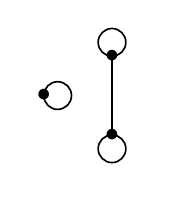
\begin{tikzpicture}[->,>=latex,node distance=1em,semithick]

\node (a2) at (0,0) {$\bullet$};
\node (b2) at (0,1) {$\bullet$};
\node (c2) at (150:1) {$\bullet$};

\node at (0.5,-0.4) {};

\path [draw,-]
    (a2.center) -- (b2.center)
    % (a.center) -- (c.center)
    % (b.center) -- (c.center)
;

\draw (a2.center) ++(-90:0.5em) circle (0.5em);
\draw (b2.center) ++(90:0.5em) circle (0.5em);
\draw (c2.center) ++(-180:-0.5em) circle (0.5em);

\end{tikzpicture}
%
        }%
    }%
    {%
        \centering%
        \subcaptionbox%
        {%
            Their product.%
            \label{Figure:ValenceGraphProductsProduct}%
        }[0.4\textwidth][c]%
        {%
            \begin{tikzpicture}[->,>=latex,node distance=1em,semithick]


    \node (a) at (0,0) {$\bullet$};
    \node (b) at (0,1) {$\bullet$};

    \node at (0.5,-0.4) {};

    \draw (a.center) ++(-90:0.5em) circle (0.5em);


    \node (a2) at (3,0) {$\bullet$};
    \node (b2) at (3,1) {$\bullet$};
    \node (c2) at ($ (3,0) + (150:1) $) {$\bullet$};

    \node at (0.5,-0.4) {};

    \path [draw,-]
        (a2.center) -- (b2.center)
        % (a.center) -- (c.center)
        % (b.center) -- (c.center)
    ;

    \draw (a2.center) ++(-90:0.5em) circle (0.5em);
    \draw (b2.center) ++(90:0.5em) circle (0.5em);
    \draw (c2.center) ++(180:-0.5em) circle (0.5em);


    \path [draw,-]
        (a.center) -- (a2.center)
        (a.center) -- (b2.center)
        (a.center) -- (c2.center)
        (b.center) -- (a2.center)
        (b.center) -- (b2.center)
        (b.center) -- (c2.center)
    ;

\end{tikzpicture}
%
        }%
    }%
    \caption{The product of a pushdown graph and a group graph.}%
    \label{Figure:ValenceGraphProducts}%
\end{figure}


\begin{example}
    \begin{thmenumerate}[a)]
        \item
            Every graph can be seen as the product of itself and the empty graph.
        \item
            The graph from \cref{Figure:ValenceSystemExamplesMPDS} is a product of two copies of the graph from \cref{Figure:ValenceSystemExamplesPDS}.
            Indeed, the storage of a multi-pushdown system consists of several fully independent stacks.
        \item
            The graph from \cref{Figure:ValenceSystemExamplesVASS} is a product of three copies of a graph consisting of a single node with no self-loop.
            Similarly, the graph from \cref{Figure:ValenceSystemExamplesIntegerVASS} is a product of three copies of a single node with a self-loop.
            Indeed, the storage of an (integer) VASS consists of several fully independent counters.
        \item
            The graph from \cref{Figure:ValenceGraphProductsProduct} is a product of the pushdown graph from \cref{Figure:ValenceGraphProductsPushdown} and the group graph from \cref{Figure:ValenceGraphProductsGroup}.
    \end{thmenumerate}
\end{example}

\begin{remark*}
    One can also define the product operation on the level of monoids.
    The \emph{(direct) product of two monoids} is a monoid whose elements are tuples consisting of an element of the first monoid and the second monoid.
    The operation on the product monoid is the component-wise application of the two monoid operations and the neutral element is the tuple of neutral elements.

    We argue that the graph monoid associated to the product of two graphs is the product of the corresponding graph monoids.
    Let $G_1$, $G_2$ be graphs and let $G_\times = G_1 \times G_2$ be their product.
    Any element of $\graphmonoid{G_\times}$ can be represented by a sequence $m_1.m_2$ such that $m_1$ exclusively contains operations for the nodes of $G_1$, similar for $m_2$ and $G_2$.
    To this end, we use that the parts of the storage corresponding to $G_1$ and $G_2$ are fully independent, meaning $o_1 \indeprel o_2$ holds for any $o$ from $G_1$ and $o_2$ from $G_2$.
    Hence, an element of $\graphmonoid{G_\times}$ can be seen as a tuple consisting of an element of $\graphmonoid{G_1}$ and an element of $\graphmonoid{G_2}$.
\end{remark*}

We call a graph $G$ the \emph{product of a pushdown and a group} if it can be written as $G_1 \times G_2$ where $G_1$ is a pushdown graph and $G_2$ is a group graph.
Correspondingly, the associated graph monoid is the product of a graph monoid associated to a pushdown graph and a group.
Unfolding the definitions, a graph $G$ being the product of a pushdown and a group means that the set of nodes of $G$ can be partitioned into $V = V_1 \dotcup V_2$ such that
(1)~there are no edges among distinct nodes in $V_1$,
(2)~all nodes in $V_2$ have a self-loop,
(3)~for every pair $o_1 \in V_1$, $o_2 \in V_2$, there is an edge $o_1 \indeprel o_2$.
The graph from \cref{Figure:ValenceGraphProductsProduct} satisfies this property.
Our classification result states that these graphs are exactly the ones for which valence coverability games are decidable.

\begin{theorem}%
\label{Theorem:ValenceCoverabilityGamesClassification}%
    Valence coverability games over graph $G$ are decidable if and only if $G$ is the product of a pushdown and a group.
\end{theorem}

Before we prove the result, we discuss its implications.
We have argued before that group graphs do not really matter when considering valence coverability games.
Hence, our classification result essentially states that even with a much weaker winning condition, context-free games are still the only decidable case.

The proof of decidability is an easy extension of the proof for the decidability of reachability games, \cref{Proposition:ValenceReachabilityGamesDecidable}.
The proof of undecidability, however, uses interesting techniques.

We show decidability by treating the pushdown part as before, while ignoring the part that belongs to the group.
The latter is sound because elements of groups are always right invertible, and the corresponding part is independent of the rest.
To show that all other cases are undecidable, we show that if the graph is not of the specified shape, we can reduce undecidable reachability games to coverability games.
The rest of this section is dedicated to making both ideas precise.

\paragraph{Valence coverability games -- The decidable case}

Assume that graph $G = (V,I)$ is the product of a pushdown and a group, where $V = P \dotcup S$ is the corresponding partitioning of the nodes.
Let us denote by $\ops_P$ and $\ops_S$ the operations for nodes in $P$ and $S$, respectively.
We have argued before that any monoid element $m$ of $\graphmonoid$ can be represented using a sequence $m_P.m_S$ with $m_ \in \ops_P^*$ and $m_S \in \ops_S^*$.
We claim that $m$ is right invertible if and only if $m_P$ is.
Indeed, the part $m_S$ that corresponds to an element of a group always has a right inverse $m_S^{-1}$ as discussed in the proof of \cref{Lemma:ValenceCoverabilityGamesGroupGraph}.
If $m_P$ has a right inverse $m_P^{-1}$, then $m_P^{-1} . m_S^{-1} \cong  m_S^{-1} .m_P^{-1}$ is a right inverse for $m_P.m_S$.
Vice versa, a right inverse for $m_P.m_S$ can be written as $m_P^{-1} . m_S^{-1}$ where $m_P^{-1}$ is a right inverse for $m_P$.
Altogether, we obtain that the part of the graph that corresponds to the group graph can be simply ignored, as in the proof of \cref{Lemma:ValenceCoverabilityGamesGroup}.
The formal construction is as follows.

\begin{proposition}
    If $G$ is the product of a pushdown and a group, valence coverability games over $G$ are decidable.
\end{proposition}

\begin{proof}
    In graph $G$, discard all nodes $S$ that correspond to the group graph.
    In the game valence system, replace all transitions labeled by $\incdec{o}$ with $o \in S$ by $\eps$-labeled transitions.
    The result is a valence coverability game over a pushdown graph that is equivalent to the valence coverability game over $G$, because the operations corresponding to the group part do not matter.

    To solve this game, we proceed as in the proof of \cref{Proposition:ValenceReachabilityGamesDecidable}.
    We first apply preprocessing to all nodes that have a self-loop.
    The result is a pushdown game in which the goal is to reach the final state with arbitrary stack content.
    This target set is regular and can be solved using Cachat's algorithm~\cite{Cachat02}, as discussed in the proof of \cref{Lemma:ValenceReachabilityGamesDecidableNoEdges}.
\end{proof}

This proves one direction of \cref{Theorem:ValenceCoverabilityGamesClassification}.

\paragraph{Valence coverability games -- The undecidable case}

Showing that valence coverability games over graph $G$ are undecidable if $G$ is not the product of a pushdown and a group is more involved.
We proceed as follows:
We identify three particular graphs for which we show undecidability.
Then, we use the fact that decidability is monotonic with respect to the induced subgraph order:
If graph $G$ contains a graph for which the problem is undecidable as an induced subgraph, then the problem for $G$ also has to be undecidable.
Finally, we show that any graph that contains none of the three graphs as an induces subgraph is the product of a pushdown and a group.

We start by considering the first of the so-called \emph{illegal graphs} for which we will show undecidability.
It is depicted in \cref{Figure:ValenceCoverabilityGamesUndecidableOne}.
It consists of two distinct nodes $x$, $y$ that have no self-loops but are connected by an edge $x \indeprel y$.

\begin{figure}[t]
    \centering%
    \begin{tikzpicture}[->,>=latex,node distance=1em,semithick]

\node (o) at (0,0) {$\bullet$};
\node (u) at (2,0) {$\bullet$};
\node (a) at (1,-1) {};

\node [left of=o] {$x$};
\node [right of=u] {$y$};

\path [draw,-]
    (o.center) -- (u.center)
;

\end{tikzpicture}
%
    \caption{The $\nth{1}$ illegal graph}.%
    \label{Figure:ValenceCoverabilityGamesUndecidableOne}%
\end{figure}

\begin{lemma}%
\label{Lemma:ValenceCoverabilityGamesUndecidableOne}%
    Valence coverability games over the \nth{1} illegal graph are undecidable.
\end{lemma}

The proof is similar to the proof of \cref{Proposition:ValenceReachabilityGamesUndecidableNoEdges}.
However, we reduce from the \emph{control-state reachability problem for two-counter machines}.
This problem consists of checking whether there is a computation that starts in $(\qinit,0,0)$ and reaches the final state $\qfinal$ with arbitrary counter values.
Formally, it is defined as follows.

\begin{problem}
    \problemtitle{Control-state reachability problem for two-counter machines}
    \probleminput{Two-counter machine $M$ with initial state $q_\init$ and final state $q_\final$.}
    \problemquestion{Is there a computation $(q_\init,0,0) \to^* (q_\final,n,m)$ for some $n,m \in \N$?}
\end{problem}

Since two-counter machines are a Turing-complete model, control-state reachability is just as undecidable as configuration reachability.

\begin{figure}[t]
    {%
        \centering%
        \subcaptionbox%
        {%
            A zero-test transition in $M$.%
            \label{Figure:ValenceCoverabilityGamesZerotestOriginal}%
        }[0.3\textwidth][c]%
        {%
            \begin{tikzpicture}[->,>=latex,node distance=7em,semithick]

\node[state] (Q) {$q$};
\node[state] (P) [right of=Q] {$p$};
\node[state,draw=none] [above of=Q,node distance=4em] {}; % invisible state to fix size

\path
    (Q) edge node [above]  {$\zeroop{x}$} (P)
;

\end{tikzpicture}
%
            % we can reuse this from the reachability game case
        }%
    }%
    {%
    \centering%
    \subcaptionbox%
        {%
            Its translation in the coverability game.%
            \label{Figure:ValenceCoverabilityGamesZerotestTranslation}%
        }[0.7\textwidth][c]%
        {%
            \begin{tikzpicture}[->,>=latex,node distance=7em,semithick]

\node[roundpos] (Q) {$q$};
\node[squarepos] (Qallhat) [right of=Q] {${\hat{q}}_\allplayer$};
\node[roundpos] (P) [right of=Qallhat] {$p$};
\node[roundpos] (Qdead) [above of=Qallhat,node distance=4em] {$q_{\text{dead}}$};

\path
    (Q) edge node [above]  {$\eps$} (Qallhat)
    (Qallhat) edge node [above] {$\eps$} (P)
    (Qallhat) edge node [right] {$\dec{x}$} (Qdead)
;

\end{tikzpicture}
%
        }%
    }%
    \caption{The translation of a zero-test transition for coverability games.}%
    \label{Figure:ValenceCoverabilityGamesZerotest}%
\end{figure}

\begin{proof}[Proof of \cref{Lemma:ValenceCoverabilityGamesUndecidableOne}]
    Assume we are given a two-counter machine $M$ as an instance of the control-state reachability problem.
    We construct an equivalent valence coverability game over the \nth{1} illegal graph.
    The construction is similar to the one in the proof of \cref{Proposition:ValenceReachabilityGamesUndecidableNoEdges}.
    We see all control states of $M$ as control states of the game valence system owned by the existential player.
    We translate a transition $q \tow{\eps} p$ in $M$ into a transition $q \tow{\eps} p$ in the valence game.
    We translate $q \tow{\incop{x}} p$ and $q \tow{\decop{x}} p$ as $q \tow{\inc{x}} p$ and $q \tow{\dec{x}} p$, respectively, similar for counter $y$.
    Note that $x$ and $y$ have no self-loops in the \nth{1} illegal graph.
    Hence, the decrements are blocking and the semantics of all aforementioned operations in $M$ and in valence coverability games coincide.

    It remains to encode zero tests.
    We replace a zero-test transition $q \tow{\zeroop{x}} p$ by a gadget consisting of several transitions and fresh control states.
    The translation is depicted in \cref{Figure:ValenceCoverabilityGamesZerotest}.
    We first go to a fresh control state ${\hat{q}}_\allplayer$ owned by the universal player using an $\eps$-labeled transition.
    In this state, the universal player can either accept that the counter value of $x$ is zero and go to state $p$.
    If the counter value is not zero, the universal player can prove this by taking an $\dec{x}$-labeled transition to a deadlock state $q_{\text{dead}}$.

    We claim that this gadget works as intended:
    The existential player can only take zero-test transitions if the current counter value is indeed zero.
    If the counter value is zero, the $\dec{x}$-labeled transition to $q_{\text{dead}}$ is not enabled as the decrement is blocking.
    The universal player has no choice but to proceed to state $p$.
    If the counter value is non-zero, the universal player can move to $q_{\text{dead}}$.
    In this deadlock state, the game gets stuck and the existential player loses.

    We use one fresh state ${\hat{q}}_\allplayer$ for every zero-test transition (but we do not reflect this in the notation to improve readability).
    We may use the same deadlock state $q_{\text{dead}}$ for all zero-test transitions.
    For zero tests of the counter $y$, we use a version of the gadgets in which the transition to $q_{\text{dead}}$ is labeled by $\dec{y}$.

    The formal proof that the existential player wins the coverability game if and only if $M$ is a yes-instance of the control-state reachability problem is as in the proof of \cref{Proposition:ValenceReachabilityGamesUndecidableNoEdges}.
\end{proof}

Our gadget from \cref{Figure:ValenceCoverabilityGamesZerotest} encoding zero tests is much simpler than the one from \cref{Figure:ValenceReachabilityGamesZerotest}.
However, the simple gadget relies on the nodes $x$, $y$ not having self-loops and the decrements being blocking.
Unlike the simple gadget, the more complex gadget in the proof of \cref{Proposition:ValenceReachabilityGamesUndecidableNoEdges} generalizes to the case of the nodes having self-loops, so we were able to reuse it in the proof of \cref{Proposition:ValenceReachabilityGamesUndecidable}.

\begin{figure}[t]
    \centering%
    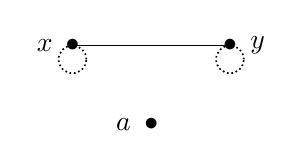
\begin{tikzpicture}[->,>=latex,node distance=1em,semithick]

\node (o) at (0,0) {$\bullet$};
\node (u) at (2,0) {$\bullet$};
\node (a) at (1,-1) {$\bullet$};

\node [left of=o] {$x$};
\node [right of=u] {$y$};
\node [left of=a] {$a$};

\path [draw,-]
    (o.center) -- (u.center)
;

\draw [densely dotted] (o.center) ++(-90:0.5em) circle (0.5em);
\draw [densely dotted] (u.center) ++(-90:0.5em) circle (0.5em);

\end{tikzpicture}
%
    \caption{The $\nth{2}$ illegal graph (or rather the set of such graphs).}%
    \label{Figure:ValenceCoverabilityGamesUndecidableTwo}%
\end{figure}

We can now consider the \nth{2} illegal graph for which we show undecidability.
It is depicted in \cref{Figure:ValenceCoverabilityGamesUndecidableTwo}.
Actually, we do not consider a single graph, but a set of graphs that are similar.
Each of the graphs consists of three nodes $x$, $y$, and $a$ such that $a$ has no self-loop, $x$ and $y$ are connected by an edge, and $a$ is connected to neither $x$ nor $y$.
Both $x$ and $y$ may or may not have a self-loop; we obtain a set of four graphs in which none, one, or both of these nodes have a self-loop.
We have depicted these self-loops that may or may not be present as dotted edges in \cref{Figure:ValenceCoverabilityGamesUndecidableTwo}.

\begin{lemma}%
\label{Lemma:ValenceCoverabilityGamesUndecidableTwo}%
    Valence coverability games over (any of the) \nth{2} illegal graph(s) are undecidable.
\end{lemma}

This time, we will not need to give a reduction from two-counter machines, although it would not be too difficult to do so.
Instead, we will be able to reduce from valence reachability games using the undecidability results that we have established in the first half of this section.

\begin{proof}
    Let $G$ be one of the \nth{2} illegal graphs.
    Consider the subgraph $G'$ induced by the set of nodes $\set{x,y}$.
    It is not a pushdown graph since $x \indeprel y$.
    By \cref{Theorem:ValenceCoverabilityGamesClassification}, reachability games over $G'$ are undecidable.
    We show that if we could solve coverability games over $G$, then we could solve reachability games over the subgraph, a contradiction.

    Consider a reachability game over the subgraph, say defined by the game valence system $(\graphmonoid{G'},Q_\allplayer \dotcup Q_\explayer, \delta, \qinit, \qfinal)$.
    We construct a new game valence system $(\graphmonoid{G},\set{{\hat{q}}_\init, {\hat{q}}_\final, {\hat{q}}_\explayer} \dotcup Q_\allplayer \dotcup Q_\explayer, \hat{\delta}, {\hat{q}}_\init, {\hat{q}}_\final)$ over $G$ as follows.
    We keep all states and most of the transitions of the original game valence system.
    Furthermore, we add three new control states, all owned by the existential player, and some transitions.

    Firstly, we add a new initial state ${\hat{q}}_\init$ and a transition ${\hat{q}}_\init \tow{\inc{a}} \qinit$ to the old one.
    Secondly, we replace every transition $q \tow{o} \qfinal$ going to the old final state by a transition $q \tow{o} {\hat{q}}_\explayer$ to ${\hat{q}}_\explayer$ with the same label.
    The state ${\hat{q}}_\explayer$ has two transitions: ${\hat{q}}_\explayer \tow{\eps} \qfinal$, an $\eps$-labeled transition to the old final state, and ${\hat{q}}_\explayer \tow{\dec{a}} {\hat{q}}_\final$, an $\dec{a}$-labeled transition to the new final state.

    The effect of the first modification is obvious: It puts an $\inc{a}$ into the storage that will be present for the rest of the play until it may be eventually canceled by the $\dec{a}$-labeled transition to ${\hat{q}}_\final'$.
    (Note that the transitions of the given reachability game do not use transitions labeled by operations for $a$.)
    The second modification kicks in whenever a play would visit the old final state~$\qfinal$.
    The existential player has the choice to either prove that the storage is empty but for the initial $\inc{a}$ by going to $q_\final'$ with $\dec{a}$.
    Alternatively, she can accept that this is currently not the case by going to $q_\final$.

    Key to the correctness of the construction is that node $a$ has no self-loop and that it is not connected by an edge to both $x$ and $y$.
    Assume that the play has entered configuration $(q_\explayer,\inc{a}.m)$, where $m$ exclusively consists of operations for the nodes $x$ and $y$.
    We have that $\inc{a}.m.\dec{a}$ is right invertible if and only if $m \cong \eps$.
    Hence, the $\dec{a}$-labeled transition can only be taken if the storage is empty but for $\inc{a}$.

    With this observation, a winning strategy for the reachability can be turned into a winning strategy for the coverability game and vice versa.
    Assume that the existential player wins the reachability game.
    We construct a strategy for the coverability game.
    We start by taking the $\inc{a}$-labeled transition to the old initial state.
    Then, we mimic the winning strategy for the reachability game.
    Whenever the play of the reachability game would visit $\qfinal$ with non-empty storage, we take the sequence of transitions $q \tow{o} {\hat{q}}_\explayer \tow{\eps} \qfinal$.
    When the play eventually visits $\qfinal$ with empty storage, we take the sequence of transitions $q \tow{o} {\hat{q}}_\explayer \tow{\dec{a}} {\hat{q}}_\final$ to the new final state.

    Vice versa, a winning strategy for the coverability game can be turned into a winning strategy for the reachability game by essentially just removing the $\inc{a}$-labeled transition at the beginning and the $\dec{a}$-labeled transition at the end.

    We have reduced the undecidable problem of solving reachability games over a graph that is not a pushdown graph to the problem of solving coverability games over the \nth{2} illegal graph.
\end{proof}

\begin{figure}[t]
    \centering%
    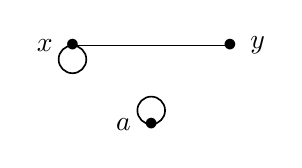
\begin{tikzpicture}[->,>=latex,node distance=1em,semithick]

\node (o) at (0,0) {$\bullet$};
\node (u) at (2,0) {$\bullet$};
\node (a) at (1,-1) {$\bullet$};

\node [left of=o] {$x$};
\node [right of=u] {$y$};
\node [left of=a] {$a$};

\path [draw,-]
    (o.center) -- (u.center)
;

\draw (o.center) ++(-90:0.5em) circle (0.5em);
\draw (a.center) ++(+90:0.5em) circle (0.5em);

\end{tikzpicture}
%
    \caption{The $\nth{3}$ illegal graph}.%
    \label{Figure:ValenceCoverabilityGamesUndecidableThree}%
\end{figure}

Finally, we consider the \nth{3} illegal graph, depicted in~\cref{Figure:ValenceCoverabilityGamesUndecidableThree}.
It consists of three nodes $x$, $y$, and $a$.
As in the \nth{2} illegal graph, $x$ and $y$ are connected by an edge.
The nodes $a$ and $x$ have self-loops while $y$ does not.


\begin{lemma}%
\label{Lemma:ValenceCoverabilityGamesUndecidableThree}%
    Valence coverability games over the \nth{3} illegal graph are undecidable.
\end{lemma}

The proof is similar to the proof for the \nth{2} illegal graph.
However, we have to extend the construction.
In the proof of \cref{Lemma:ValenceCoverabilityGamesUndecidableTwo}, we have used that $\inc{a}.m.\dec{a}$ is right invertible if and only if $m \cong \eps$.
This fact relies on node $a$ not having a self-loop, which makes the $\dec{a}$ operation blocking.
Since $a$ has a self-loop in the \nth{3} illegal graph, using $\inc{a}$ at the beginning of the play will be sufficient.
Instead, we will use $\inc{y}.\inc{a}$ at the beginning and $\dec{a}.\dec{y}$ at the end.

\begin{proof}[Proof of \cref{Lemma:ValenceCoverabilityGamesUndecidableThree}]
    Consider the subgraph of the \nth{3} illegal graph induced by the set of nodes $\set{x,y}$.
    Assume we are given a valence reachability game for this subgraph.
    Note that solving such games is undecidable by \cref{Theorem:ValenceReachabilityGamesClassification}.

    We construct a valence coverability game over the \nth{3} illegal graph as follows.
    We make sure that every play starts with the transitions $\tow{\inc{y}} \tow{\inc{a}}$ before going to the initial state of the given game
    To this end, we insert a new initial state and another fresh state as in the proof of \cref{Lemma:ValenceCoverabilityGamesUndecidableTwo}.

    Whenever there is a transition $q \tow{o} \qfinal$ entering the final state in the given game, we give the existential player the choice to either go to the old final state with operation $o$, or whether to go to the new final state using a sequence of transitions $\tow{\ o\ } \tow{\dec{a}} \tow{\dec{y}}$.

    We argue that this construction is correct.
    Every play of the coverability game that reaches the new final state does so with a sequence of storage operations of the shape $\inc{y}.\inc{a}.m.\dec{a}.\dec{y}$, where $m$ exclusively consists of operations over $x$ and $y$.
    We claim that the final $\dec{y}$ transition is enabled if and only if $m \cong \eps$.
    Obviously, $m \cong \eps$ implies that $\inc{y}.\inc{a}.m.\dec{a}.\dec{y} \cong \inc{y}.\inc{a}.\dec{a}.\dec{y} \cong \inc{y}.\dec{y} \cong \eps$ is right invertible.

    For the other direction, assume that $m$ is not equivalent to $\eps$.
    In this case, $\inc{a}.m.\dec{a}$ is not equivalent to $\eps$.
    Here, we use that $\inc{a}$ and $\dec{a}$ cannot be swapped with any of the operations in $m$ since $a \notindeprel x$ and $a \notindeprel y$.
    If $\inc{a}.m.\dec{a}$ is not equivalent to $\eps$, then $\inc{y}\inc{a}.m.\dec{a}$ is not equivalent to any sequence of operations that ends with $\inc{y}$
    Since $a \notindeprel y$ we can neither swap the $\inc{y}$ from the beginning to the end, nor can we swap any $\inc{y}$ that might be contained in $m$ to the end.
    Consequently, $\inc{y}.\inc{a}.m.\dec{a}.\dec{y}$ is not right invertible.
    The final $\dec{y}$ cannot be canceled using an $\inc{y}$ operation in the prefix $\inc{y}.\inc{a}.m.\dec{a}$ as argued before.
    Furthermore, it can also not be canceled by a hypothetical later occurrence of an $\inc{y}$ operation.
    Node~$y$ has no self-loop, so $\inc{y}$ is not the right inverse of $\dec{y}$.

    One can now prove that the new coverability game is equivalent to the reachability game.
    The details are as in the proof of \cref{Lemma:ValenceCoverabilityGamesUndecidableTwo}.
\end{proof}

Before proving the result, we formally observe that decidability is monotonic with respect to the induced subgraph order.

\begin{lemma}%
\label{Lemma:ValenceCoverabilityGamesUndecidableInduced}%
    If graph $G$ contains any of the three illegal graphs as an induced subgraph, valence coverability games over $G$ are undecidable.
\end{lemma}

\begin{proof}
    Using the \cref{Lemma:ValenceCoverabilityGamesUndecidableOne,,Lemma:ValenceCoverabilityGamesUndecidableTwo,,Lemma:ValenceCoverabilityGamesUndecidableThree}, we know that valence coverability games over the illegal graphs are undecidable.
    Assume $G$ contains one of the illegal graphs as an induced subgraph.
    Valence coverability games for that subgraph can be seen as valence coverability games over graph $G$ that do not use the operations for any nodes not contained in the subgraph.
    If we could decide coverability games over graph $G$, we could also solve coverability games for the subgraph, a contradiction.
\end{proof}

We can finally prove the remaining implication for \cref{Theorem:ValenceCoverabilityGamesClassification}.

\begin{proposition}%
\label{Proposition:ValenceCoverabilityGamesUndecidable}
    If graph $G$ is not the product of a pushdown and a group, valence coverability games over $G$ are undecidable.
\end{proposition}

Using \cref{Lemma:ValenceCoverabilityGamesUndecidableInduced}, it is sufficient to show that any graph that is not the product of a pushdown and a group contains one of the illegal graphs as induced subgraph.
We use contraposition and show that if a graph does not contain one of the illegal graphs, then it has to be the product of a pushdown and a group.
We start with a general graph that may or may not contain any edge that is not a self-loop.
Then, we iteratively show the existence or non-existence of some edges, until we obtain a graph that is the product of a pushdown and a group.

The most accessible version of this proof is via a sequence of pictures, \cref{Figure:ValenceCoverabilityGamesUndecidableProof}.
For the sake of completeness, we also provide a formal write-up below.

\begin{figure}
    {%
        \centering%
        \subcaptionbox*%
        {%
            \nth{1} illegal graph.%
        }%
        [0.32\textwidth][c]%
        {%
            \begin{tikzpicture}[->,>=latex,node distance=1em,semithick]

\node (o) at (0,0) {$\bullet$};
\node (u) at (2,0) {$\bullet$};
\node (a) at (1,-1) {};

\node [left of=o] {$x$};
\node [right of=u] {$y$};

\path [draw,-]
    (o.center) -- (u.center)
;

\end{tikzpicture}
%
        }%
    }%
    {%
        \centering%
        \subcaptionbox*%
        {%
            \nth{2} illegal graph.%
        }%
        [0.32\textwidth][c]%
        {%
            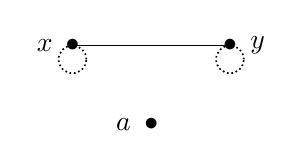
\begin{tikzpicture}[->,>=latex,node distance=1em,semithick]

\node (o) at (0,0) {$\bullet$};
\node (u) at (2,0) {$\bullet$};
\node (a) at (1,-1) {$\bullet$};

\node [left of=o] {$x$};
\node [right of=u] {$y$};
\node [left of=a] {$a$};

\path [draw,-]
    (o.center) -- (u.center)
;

\draw [densely dotted] (o.center) ++(-90:0.5em) circle (0.5em);
\draw [densely dotted] (u.center) ++(-90:0.5em) circle (0.5em);

\end{tikzpicture}
%
        }%
    }%
    {%
        \centering%
        \subcaptionbox*%
        {%
            \nth{3} illegal graph.%
        }%
        [0.32\textwidth][c]%
        {%
            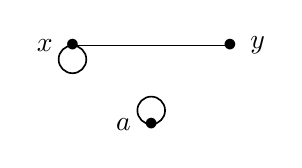
\begin{tikzpicture}[->,>=latex,node distance=1em,semithick]

\node (o) at (0,0) {$\bullet$};
\node (u) at (2,0) {$\bullet$};
\node (a) at (1,-1) {$\bullet$};

\node [left of=o] {$x$};
\node [right of=u] {$y$};
\node [left of=a] {$a$};

\path [draw,-]
    (o.center) -- (u.center)
;

\draw (o.center) ++(-90:0.5em) circle (0.5em);
\draw (a.center) ++(+90:0.5em) circle (0.5em);

\end{tikzpicture}
%
        }%
    }%
    \caption*{Recall: The three illegal graphs.}%
    \vspace*{1em}
    {%
        \centering%
        \subcaptionbox%
        {%
            A general graph in which some nodes (the~$s_j$) have self-loops while others (the~$e_i$) do not. All dotted edges may or may not exist.
            If any of the thick dashed edges among the $e_i$ exists, the graph contains the \nth{1} illegal graph.%
            \label{Figure:ValenceCoverabilityGamesUndecidableProofOne}%
        }%
        [0.45\textwidth][c]%
        {%
            \begin{tikzpicture}[->,>=latex,node distance=1em,semithick,scale=0.75]

\CoverabilityGamesUndecidableVisualProofBasicSetup

% edges among the ei (left row)
\path [densely dashed,-,very thick]
    (e1.center) edge (e2.center)
    (e2.center) edge (e3.center)
    (e1.center) edge [bend right, looseness=1.4] (e3.center)
;
% edges among the sj (middle row)
\path [densely dotted,-]
    (s1.center) edge (s2.center)
    (s2.center) edge (s3.center)
    (s1.center) edge [bend right, looseness=1.4] (s3.center)
;
% edges among the sl (right row)
\path [densely dotted,-]
    (s4.center) edge (s5.center)
    (s5.center) edge (s6.center)
    (s4.center) edge [bend left, looseness=1.4] (s6.center)
;
% edges from the ei (left row) to the sj (middle row)
\path [densely dotted,-]
    (e1.center) edge (s1.center)
    (e1.center) edge (s2.center)
    (e1.center) edge (s3.center)
    (e2.center) edge (s1.center)
    (e2.center) edge (s2.center)
    (e2.center) edge (s3.center)
    (e3.center) edge (s1.center)
    (e3.center) edge (s2.center)
    (e3.center) edge (s3.center)
;
% edges from the ei (left row) to the sj (right row)
\path [densely dotted,-]
    (e1.center) edge [bend left] (s4.center)
    (e1.center) edge (s5.center)
    (e1.center) edge (s6.center)
    (e2.center) edge (s4.center)
    (e2.center) edge [bend right,looseness=0.7] (s5.center)
    (e2.center) edge (s6.center)
    (e3.center) edge (s4.center)
    (e3.center) edge (s5.center)
    (e3.center) edge [bend right] (s6.center)
;
% edges from the sj (middle row) to the sj (right row)
\path [densely dotted,-]
    (s1.center) edge (s4.center)
    (s1.center) edge (s5.center)
    (s1.center) edge (s6.center)
    (s2.center) edge (s4.center)
    (s2.center) edge (s5.center)
    (s2.center) edge (s6.center)
    (s3.center) edge (s4.center)
    (s3.center) edge (s5.center)
    (s3.center) edge (s6.center)
;

\end{tikzpicture}
%
        }%
    }%
    \hspace*{0.1\textwidth}%
    {%
        \centering%
        \subcaptionbox%
        {%
            If any of the thick dashed edges from the $e_i$ to $s_1$ exists, all of them have to exist.
            Otherwise, the graph would contain the \nth{2} illegal graph.
            A similar reasoning holds for all $s_j$.%
            \label{Figure:ValenceCoverabilityGamesUndecidableProofTwo}%
        }%
        [0.45\textwidth][c]%
        {%
            \begin{tikzpicture}[->,>=latex,node distance=1em,semithick,scale=0.75]

    \CoverabilityGamesUndecidableVisualProofBasicSetup

    % edges among the ei (left row)
    % \path [densely dotted,-,very thick]
    %     (e1.center) edge (e2.center)
    %     (e2.center) edge (e3.center)
    %     (e1.center) edge [bend right, looseness=1.4] (e3.center)
    % ;
    % edges among the sj (middle row)
    \path [densely dotted,-]
        (s1.center) edge (s2.center)
        (s2.center) edge (s3.center)
        (s1.center) edge [bend right, looseness=1.4] (s3.center)
    ;
    % edges among the sl (right row)
    \path [densely dotted,-]
        (s4.center) edge (s5.center)
        (s5.center) edge (s6.center)
        (s4.center) edge [bend left, looseness=1.4] (s6.center)
    ;
    % edges from the ei (left row) to the sj (middle row)
    \path [densely dotted,-]
        (e1.center) edge [densely dashed, very thick] (s1.center)
        (e1.center) edge (s2.center)
        (e1.center) edge (s3.center)
        (e2.center) edge [densely dashed, very thick]  (s1.center)
        (e2.center) edge (s2.center)
        (e2.center) edge (s3.center)
        (e3.center) edge [densely dashed, very thick]  (s1.center)
        (e3.center) edge (s2.center)
        (e3.center) edge (s3.center)
    ;
    % edges from the ei (left row) to the sj (right row)
    \path [densely dotted,-]
        (e1.center) edge [bend left] (s4.center)
        (e1.center) edge (s5.center)
        (e1.center) edge (s6.center)
        (e2.center) edge (s4.center)
        (e2.center) edge [bend right,looseness=0.7] (s5.center)
        (e2.center) edge (s6.center)
        (e3.center) edge (s4.center)
        (e3.center) edge (s5.center)
        (e3.center) edge [bend right] (s6.center)
    ;
    % edges from the sj (middle row) to the sj (right row)
    \path [densely dotted,-]
        (s1.center) edge (s4.center)
        (s1.center) edge (s5.center)
        (s1.center) edge (s6.center)
        (s2.center) edge (s4.center)
        (s2.center) edge (s5.center)
        (s2.center) edge (s6.center)
        (s3.center) edge (s4.center)
        (s3.center) edge (s5.center)
        (s3.center) edge (s6.center)
    ;

    \end{tikzpicture}
%
        }%
    }%
    \\[0.75em]%
    {%
        \centering%
        \subcaptionbox%
        {%
            Hence, some of the $s_j$ ($S_g = \set{s_1, s_2, s_3}$) are adjacent to all $e_i$ while the others ($S_p = \set{s_4, s_5, s_6}$) are not adjacent to any $e_i$.%
            \label{Figure:ValenceCoverabilityGamesUndecidableProofThree}%
        }%
        [0.45\textwidth][c]%
        {%
            \begin{tikzpicture}[->,>=latex,node distance=1em,semithick,scale=0.75]

    \CoverabilityGamesUndecidableVisualProofBasicSetup

    % edges among the ei (left row)
    % \path [densely dotted,-,very thick]
    %     (e1.center) edge (e2.center)
    %     (e2.center) edge (e3.center)
    %     (e1.center) edge [bend right, looseness=1.4] (e3.center)
    % ;
    % edges among the sj (middle row)
    \path [densely dotted,-]
        (s1.center) edge (s2.center)
        (s2.center) edge (s3.center)
        (s1.center) edge [bend right, looseness=1.4] (s3.center)
    ;
    % edges among the sl (right row)
    \path [densely dotted,-]
        (s4.center) edge (s5.center)
        (s5.center) edge (s6.center)
        (s4.center) edge [bend left, looseness=1.4] (s6.center)
    ;
    % edges from the ei (left row) to the sj (middle row)
    \path [-]
        (e1.center) edge (s1.center)
        (e1.center) edge (s2.center)
        (e1.center) edge (s3.center)
        (e2.center) edge (s1.center)
        (e2.center) edge (s2.center)
        (e2.center) edge (s3.center)
        (e3.center) edge (s1.center)
        (e3.center) edge (s2.center)
        (e3.center) edge (s3.center)
    ;
    % % edges from the ei (left row) to the sj (right row)
    % \path [densely dotted,-]
    %     (e1.center) edge [bend left] (s4.center)
    %     (e1.center) edge (s5.center)
    %     (e1.center) edge (s6.center)
    %     (e2.center) edge (s4.center)
    %     (e2.center) edge [bend right,looseness=0.7] (s5.center)
    %     (e2.center) edge (s6.center)
    %     (e3.center) edge (s4.center)
    %     (e3.center) edge (s5.center)
    %     (e3.center) edge [bend right] (s6.center)
    % ;
    % edges from the sj (middle row) to the sj (right row)
    \path [densely dotted,-]
        (s1.center) edge (s4.center)
        (s1.center) edge (s5.center)
        (s1.center) edge (s6.center)
        (s2.center) edge (s4.center)
        (s2.center) edge (s5.center)
        (s2.center) edge (s6.center)
        (s3.center) edge (s4.center)
        (s3.center) edge (s5.center)
        (s3.center) edge (s6.center)
    ;

    \end{tikzpicture}
%
        }%
    }%
    \hspace*{0.1\textwidth}%
    {%
        \centering%
        \subcaptionbox%
        {%
            If any of the thick dashed edges among the nodes in $S_p = \set{s_4, s_5, s_6}$ exists, the graph contains the \nth{2} illegal graph%
            \label{Figure:ValenceCoverabilityGamesUndecidableProofFour}%
        }%
        [0.45\textwidth][c]%
        {%
            \begin{tikzpicture}[->,>=latex,node distance=1em,semithick,scale=0.75]

    \CoverabilityGamesUndecidableVisualProofBasicSetup

    % edges among the ei (left row)
    % \path [densely dotted,-,very thick]
    %     (e1.center) edge (e2.center)
    %     (e2.center) edge (e3.center)
    %     (e1.center) edge [bend right, looseness=1.4] (e3.center)
    % ;
    % edges among the sj (middle row)
    \path [densely dotted,-]
        (s1.center) edge (s2.center)
        (s2.center) edge (s3.center)
        (s1.center) edge [bend right, looseness=1.4] (s3.center)
    ;
    % edges among the sl (right row)
    \path [densely dashed,-,very thick]
        (s4.center) edge (s5.center)
        (s5.center) edge (s6.center)
        (s4.center) edge [bend left, looseness=1.4] (s6.center)
    ;
    % edges from the ei (left row) to the sj (middle row)
    \path [-]
        (e1.center) edge (s1.center)
        (e1.center) edge (s2.center)
        (e1.center) edge (s3.center)
        (e2.center) edge (s1.center)
        (e2.center) edge (s2.center)
        (e2.center) edge (s3.center)
        (e3.center) edge (s1.center)
        (e3.center) edge (s2.center)
        (e3.center) edge (s3.center)
    ;
    % % edges from the ei (left row) to the sj (right row)
    % \path [densely dotted,-]
    %     (e1.center) edge [bend left] (s4.center)
    %     (e1.center) edge (s5.center)
    %     (e1.center) edge (s6.center)
    %     (e2.center) edge (s4.center)
    %     (e2.center) edge [bend right,looseness=0.7] (s5.center)
    %     (e2.center) edge (s6.center)
    %     (e3.center) edge (s4.center)
    %     (e3.center) edge (s5.center)
    %     (e3.center) edge [bend right] (s6.center)
    % ;
    % edges from the sj (middle row) to the sj (right row)
    \path [densely dotted,-]
        (s1.center) edge (s4.center)
        (s1.center) edge (s5.center)
        (s1.center) edge (s6.center)
        (s2.center) edge (s4.center)
        (s2.center) edge (s5.center)
        (s2.center) edge (s6.center)
        (s3.center) edge (s4.center)
        (s3.center) edge (s5.center)
        (s3.center) edge (s6.center)
    ;

    \end{tikzpicture}
%
        }%
    }%
    \\[0.75em]%
    {%
        \centering%
        \subcaptionbox%
        {%
            If any of the thick dashed edges from $S_g = \set{s_1, s_2, s_3}$ to $S_p = \set{s_4, s_5, s_6}$ is missing, the graph contains the \nth{3} illegal graph.%
            \label{Figure:ValenceCoverabilityGamesUndecidableProofFive}%
        }%
        [0.45\textwidth][c]%
        {%
            \begin{tikzpicture}[->,>=latex,node distance=1em,semithick,scale=0.75]

    \CoverabilityGamesUndecidableVisualProofBasicSetup

    % edges among the ei (left row)
    % \path [densely dotted,-,very thick]
    %     (e1.center) edge (e2.center)
    %     (e2.center) edge (e3.center)
    %     (e1.center) edge [bend right, looseness=1.4] (e3.center)
    % ;
    % edges among the sj (middle row)
    \path [densely dotted,-]
        (s1.center) edge (s2.center)
        (s2.center) edge (s3.center)
        (s1.center) edge [bend right, looseness=1.4] (s3.center)
    ;
    % edges among the sl (right row)
    % \path [densely dotted,-,very thick]
    %     (s4.center) edge (s5.center)
    %     (s5.center) edge (s6.center)
    %     (s4.center) edge [bend left, looseness=1.4] (s6.center)
    % ;
    % edges from the ei (left row) to the sj (middle row)
    \path [-]
        (e1.center) edge (s1.center)
        (e1.center) edge (s2.center)
        (e1.center) edge (s3.center)
        (e2.center) edge (s1.center)
        (e2.center) edge (s2.center)
        (e2.center) edge (s3.center)
        (e3.center) edge (s1.center)
        (e3.center) edge (s2.center)
        (e3.center) edge (s3.center)
    ;
    % % edges from the ei (left row) to the sj (right row)
    % \path [densely dotted,-]
    %     (e1.center) edge [bend left] (s4.center)
    %     (e1.center) edge (s5.center)
    %     (e1.center) edge (s6.center)
    %     (e2.center) edge (s4.center)
    %     (e2.center) edge [bend right,looseness=0.7] (s5.center)
    %     (e2.center) edge (s6.center)
    %     (e3.center) edge (s4.center)
    %     (e3.center) edge (s5.center)
    %     (e3.center) edge [bend right] (s6.center)
    % ;
    % edges from the sj (middle row) to the sj (right row)
    \path [densely dashed,-,very thick]
        (s1.center) edge (s4.center)
        (s1.center) edge (s5.center)
        (s1.center) edge (s6.center)
        (s2.center) edge (s4.center)
        (s2.center) edge (s5.center)
        (s2.center) edge (s6.center)
        (s3.center) edge (s4.center)
        (s3.center) edge (s5.center)
        (s3.center) edge (s6.center)
    ;

    \end{tikzpicture}
%
        }%
    }%
    \hspace*{0.1\textwidth}%
    {%
        \centering%
        \subcaptionbox%
        {%
            The resulting graph is the product of a pushdown with nodes $\set{e_1,e_2,e_3,s_4,s_5,s_6}$ and a group with nodes $\set{s_1,s_2,s_3}$.
            Dotted edges among $\set{s_1,s_2,s_3}$ may or may not exist.%
            \label{Figure:ValenceCoverabilityGamesUndecidableProofSix}%
        }%
        [0.45\textwidth][c]%
        {%
            \begin{tikzpicture}[->,>=latex,node distance=1em,semithick,scale=0.75]

    \CoverabilityGamesUndecidableVisualProofBasicSetup

    % edges among the ei (left row)
    % \path [densely dotted,-,very thick]
    %     (e1.center) edge (e2.center)
    %     (e2.center) edge (e3.center)
    %     (e1.center) edge [bend right, looseness=1.4] (e3.center)
    % ;
    % edges among the sj (middle row)
    \path [densely dotted,-]
        (s1.center) edge (s2.center)
        (s2.center) edge (s3.center)
        (s1.center) edge [bend right, looseness=1.4] (s3.center)
    ;
    % edges among the sl (right row)
    % \path [densely dotted,-,very thick]
    %     (s4.center) edge (s5.center)
    %     (s5.center) edge (s6.center)
    %     (s4.center) edge [bend left, looseness=1.4] (s6.center)
    % ;
    % edges from the ei (left row) to the sj (middle row)
    \path [-]
        (e1.center) edge (s1.center)
        (e1.center) edge (s2.center)
        (e1.center) edge (s3.center)
        (e2.center) edge (s1.center)
        (e2.center) edge (s2.center)
        (e2.center) edge (s3.center)
        (e3.center) edge (s1.center)
        (e3.center) edge (s2.center)
        (e3.center) edge (s3.center)
    ;
    % % edges from the ei (left row) to the sj (right row)
    % \path [densely dotted,-]
    %     (e1.center) edge [bend left] (s4.center)
    %     (e1.center) edge (s5.center)
    %     (e1.center) edge (s6.center)
    %     (e2.center) edge (s4.center)
    %     (e2.center) edge [bend right,looseness=0.7] (s5.center)
    %     (e2.center) edge (s6.center)
    %     (e3.center) edge (s4.center)
    %     (e3.center) edge (s5.center)
    %     (e3.center) edge [bend right] (s6.center)
    % ;
    % edges from the sj (middle row) to the sj (right row)
    \path [-]
        (s1.center) edge (s4.center)
        (s1.center) edge (s5.center)
        (s1.center) edge (s6.center)
        (s2.center) edge (s4.center)
        (s2.center) edge (s5.center)
        (s2.center) edge (s6.center)
        (s3.center) edge (s4.center)
        (s3.center) edge (s5.center)
        (s3.center) edge (s6.center)
    ;

    \end{tikzpicture}
%
        }%
    }%
    \caption{The proof of \cref{Proposition:ValenceCoverabilityGamesUndecidable} in pictures.}%
    \label{Figure:ValenceCoverabilityGamesUndecidableProof}%
\end{figure}


\begin{proof}
    Using \cref{Lemma:ValenceCoverabilityGamesUndecidableInduced} and contraposition, it is sufficient to show that any graph that does not contain an illegal graph is the product of a pushdown and a group.

    We proceed in several steps.
    The enumeration corresponds to the subfigures of \cref{Figure:ValenceCoverabilityGamesUndecidableProof}.

    \begin{enumerate}[i)]
        \item
            Consider an arbitrary graph $(V,I)$.
            We may partition $V = E \dotcup S$ so that each $s_j \in S$ has a self-loop, $s_j \indeprel s_j$, and each $e_i \in E$ does not, $e_i \notindeprel e_i$.
            All edges among distinct nodes may or may not exist.

            If the set $E$ is empty, the graph is a group graph.
            Hence, it is the product of itself and an empty pushdown graph.
            It satisfies the requirements and we are done.
            In the following, we assume that there is at least one $e_i \in E$.

            If there are two distinct $e_i, e_{i'} \in E$, $e_i \neq e_{i'}$ that are connected by an edge, $e_i \indeprel e_{i'}$, the graph contains the \nth{1} illegal graph as induced subgraph.
            To see this, define $x = e_i$ and $y = e_{i'}$.
            Hence, we may restrict ourselves to graphs in which there is no edge among the nodes in~$E$.

            If the set $S$ is empty, we have shown that the graph is a pushdown graph.
            Hence, it is the product of itself and an empty group graph, and we are done.
            In the following, we will assume that there is at least one $s_j \in S$.
        \item
            If some $s_j \in S$ is adjacent to at least one $e_i \in E$, $e_i \indeprel s_j$, this $s_j$ needs to be adjacent to all~$e_i$.
            This property is trivially satisfied if there is just a single $E = \set{e_i}$.
            Otherwise, consider distinct elements $e_i, e_{i'} \in E$ and assume $e_{i'} \notindeprel s_j$.
            By defining $x = e_i$, $y = s_j$ and $a = e_{i'}$, we see that the graph would contain the \nth{2} illegal graph  as induced subgraph.
        \item
            The previously stated property holds for all elements of $S$.
            Hence, we may partition $S = S_g \dotcup S_p$ such that the $s_g \in S_g$ are adjacent to all $e_i \in E$ while the $s_p \in S_p$ are not adjacent to any $e_i \in E$.
        \item
            If $S_p$ contains distinct elements $s_p, s_{p'}$ that are connected by an edge, $s_p \indeprel s_{p'}$, the graph would contain the \nth{2} illegal graph as induced subgraph.
            To see this, consider $e_i \in E$  and note that it is not adjacent to any element of $S_p$.
            We may set $a = e_i$, $x = s_p$ and $y = s_{p'}$ to identify the \nth{2} illegal graph.
        \item
            If the set $S_g$ is empty, the graph is a pushdown graph and we are done.
            Indeed, there are no edges among the nodes in $E$, see Step~i), no edges among the nodes in $S_p$, see Step~iv), and no edges that connect an element of $E$ to an element of $S_p$, see Step~ii).
            Hence, assume that $S_g$ is non-empty.

            If the set $S_p$ is empty, the graph is a product of a group and a pushdown and we are done.
            The pushdown graph consists of the set of nodes $E$, while the group graph consists of the set of nodes $S_g$.
            Indeed, there are no edges among the elements of $E$, each node in $S_g$ has a self-loop, and every $e_i \in E$ is adjacent to every $s_g \in S_g$.
            Hence, assume that $S_p$ is non-empty.

            We claim that every $s_p \in S_p$ needs to be adjacent to every $s_g \in S_g$.
            Assume that $s_p \notindeprel s_g$ holds.
            Then we can identify the \nth{3} illegal graph as an induced subgraph by defining $x = s_g$, $a = s_p$, and $y = e_i$ for some $e_i \in E$.
            Indeed, $s_g$ is adjacent to $e_i$ but $s_p$ is not.
        \item
            We obtain a graph with set of nodes $E \dotcup S_g \dotcup S_p$.
            We claim this graph is the product of a pushdown and a group.
            The set of nodes belonging to the pushdown graph is $E \dotcup S_p$ while the nodes in $S_g$ belong to the group graph.
            Indeed, there are no edges among the nodes in $E \dotcup S_p$, see Steps~i),~ii)~and~iv).
            Furthermore, each $s_g \in S_g$ is adjacent to any node is $E \dotcup S_p$, see Steps~iv)~and~v).
            The edges in $S_g \subseteq S$ have self-loops.
            Edges among the $S_g$ may or may not exist.
    \end{enumerate}
    \vspace*{-2.5em}
\end{proof}

\cref{Proposition:ValenceCoverabilityGamesUndecidable} shows the missing direction for the proof of our classification result, \cref{Theorem:ValenceCoverabilityGamesClassification}.
This completes our study of valence reachability and coverability games.

\end{document}
